\documentclass[11pt,a4paper]{article}
\usepackage[margin=2.4cm]{geometry}
\usepackage{microtype}
\usepackage{booktabs,tabularx,longtable,array}
\usepackage{enumitem}
\usepackage{graphicx}
\usepackage{xcolor}
\usepackage{amsmath}
\usepackage{tikz}
\usetikzlibrary{positioning,arrows.meta}
\usepackage[hidelinks]{hyperref}
\usepackage{url}
\def\UrlBreaks{\do\/\do\-\do\_}
\usepackage{caption}
\captionsetup{font=small,labelfont=bf}
\setlist{itemsep=3pt,topsep=5pt}
\setlength{\parskip}{6pt}
\setlength{\parindent}{0pt}
\emergencystretch=2em
\renewcommand{\arraystretch}{1.35}
\newcolumntype{L}[1]{>{\raggedright\arraybackslash}p{#1}}
\newcommand{\code}[1]{\texttt{#1}}

\title{\textbf{RouteTwin NG}\\[3pt]\large A digital twin of a smart road: tracking pavement health, traffic and\\maintenance needs on the Lagos--Ibadan expressway}
\author{Dominum\\ Department of Mechatronics Engineering, Federal University Oye-Ekiti, Nigeria}
\date{ISA Nigeria Section Next-Gen Automation Challenge\\Proposal, November 2026}

\begin{document}
\maketitle

\begin{abstract}
Heavy trucks are a major cause of road wear, yet those responsible for maintaining roads rarely have continuous information about the damage accumulated by each section since its last inspection. Potholes can develop and traffic queues can form without being detected until a driver reports them. This proposal presents RouteTwin NG, a digital twin of the Lagos--Ibadan expressway that treats the corridor as a smart road comprising thirteen instrumented segments. The system continuously estimates pavement condition, remaining service life, and traffic conditions. Roadside stations report traffic volumes, truck axle loads, and pavement temperatures, while instrumented trucks provide roughness measurements as they travel along the road. A Kalman filter for each segment combines a load-driven wear model with these roughness measurements, estimates the structural response of each segment, and supports alarms, rerouting advice, and a prioritised maintenance queue. The alarm system is designed around ISA-18.2, the operator interface follows ISA-101 principles, and the data interfaces implement selected security requirements from IEC 62443. The proposal is accompanied by a working prototype that runs locally with a single command, an interactive 3D dashboard in which up to three scenarios can be simulated together, and 61 automated tests. All reported results are based on simulation. They demonstrate that the twin behaves as specified by its models, but do not establish that it accurately represents real Nigerian roads. A model-mismatch test shows that the absolute condition estimate depends strongly on how the roughness-to-condition relationship is calibrated, and the proposal identifies the fieldwork required to establish that calibration and to assess real-world performance.
\end{abstract}

\subsection*{How to read this proposal}
Each section begins by explaining the problem or concept, then introduces the relevant engineering principles, and finally presents the equations, parameters, and logic. Each reported result is assigned one of three labels.

\begin{center}
\small
\begin{tabularx}{\textwidth}{@{}L{2.4cm} X@{}}
\toprule
\textbf{Verified} & Checked using an automated test or script against analytical properties or hidden simulated ground truth.\\[3pt]
\textbf{Simulated} & Generated by the seeded simulator using illustrative parameters. These results demonstrate the design's behaviour, not the behaviour of real roads.\\[3pt]
\textbf{Planned} & To be measured during the field pilot described in Section~\ref{sec:workability}. No field measurements are available yet.\\
\bottomrule
\end{tabularx}
\end{center}

%==========================================================================
\section{The problem}
\subsection{Challenges in Road Condition Monitoring and Maintenance}
Road deterioration is closely related to the loads imposed on the pavement, with heavy trucks generally causing substantially more damage than passenger cars. Overloaded trucks can accelerate pavement deterioration disproportionately, even when axle loads increase by relatively small amounts. However, road authorities often become aware of deterioration only after visible damage has developed. Between routine inspections, information may be limited about which road sections are deteriorating most rapidly, where new potholes have formed, or where traffic congestion has emerged. Consequently, maintenance is often scheduled according to fixed timetables or initiated only after damage has become severe. Similarly, drivers and fleet dispatchers may learn about road blockages and other disruptions only through reports from other road users, leading to delayed responses and inefficient route planning.

\subsection{Industry, process, and asset}
The industry addressed by this proposal is road freight and the infrastructure that supports it. The process of interest is the movement of goods along the Lagos--Ibadan expressway, a major route connecting the Lagos ports region with inland destinations, together with the maintenance of its pavement. The asset modelled is the pavement itself, divided into thirteen segments ranging from 4.9 to 14.5~km in length, with two or three lanes in each direction.

The underlying damage mechanism is nonlinear. Pavement engineers express the wear caused by vehicles in terms of equivalent standard axle loads (ESALs), which represent the number of passes by a reference 80~kN axle that would cause equivalent damage. The AASHTO guide approximates this relationship using a fourth-power law: an axle load that is 10\% heavier produces approximately 46\% more damage per pass than the reference load \cite{aashto}.

\subsection{Evidence from Nigerian and international studies}
Studies of Nigerian roads report substantial pavement overstress. An axle-load survey conducted by the Nigerian Building and Road Research Institute on the Gombe--Numan expressway found loading levels of approximately five times the standard axle load and recommended the use of weigh-in-motion stations and routine axle-load surveys \cite{nbrri}. Research on goods haulage in Nigeria also emphasises the need for stricter control of truck loads \cite{oguntayo}, while international evidence shows that overloaded vehicles increase pavement damage and life-cycle costs relative to legally loaded vehicles \cite{pais}. Trade publications have described the Apapa--Oshodi expressway, a major route serving the ports, as having severely deteriorated because of age, neglect, and heavy truck traffic \cite{shippingposition}. This road also connects to the Lagos--Ibadan expressway \cite{businessday}.

None of these sources directly measures the condition of the Lagos--Ibadan expressway, and we found no publicly available, corridor-specific data on axle loads or pavement condition. Generating such data is therefore a primary objective of the pilot described in Section~\ref{sec:workability}.

\subsection{Why current approaches fall short}
\begin{itemize}
\item Road condition is assessed mainly through periodic surveys. Deterioration between surveys, newly formed potholes, and increases in overloaded truck traffic can therefore remain undetected until visible damage occurs.
\item Maintenance is often driven by fixed schedules or existing failures rather than measured pavement condition and the estimated remaining life of individual road sections.
\item Drivers typically identify slow or blocked sections after encountering them, meaning that warnings may reach approaching trucks too late to support effective rerouting.
\item In our assessment, the public data sources we examined---including the FRSC road safety observatory, FERMA GIS layers, the free tier of a commercial traffic service, and the national weather service API---cannot yet be relied upon to support this corridor. Some provide little useful information for Nigerian expressways, while others show no recent activity. We did not conduct a formal access audit. Accordingly, the proposed design treats external data feeds as optional and defines a common data contract through which suitable sources can be integrated later.
\end{itemize}

\subsection{Measurable objectives}
\begin{center}
\small
\begin{tabularx}{\textwidth}{@{}L{1.0cm} X L{5.2cm}@{}}
\toprule
 & Objective & Status\\
\midrule
O1 & Continuously estimate the condition index (CI) of each segment, with low error relative to hidden ground truth & Verified in simulation: mean absolute CI error of 0.2 to 0.5 points when the twin's model matches the truth (Section~\ref{sec:results})\\[4pt]
O2 & Detect and locate potholes from roughness readings without generating false entries & Verified in simulation: the registry matched ground truth across all 13 segments over 30 days\\[4pt]
O3 & Detect severe congestion (speeds below 10 km/h) and closures, and raise alarms designed around ISA-18.2 \cite{isa182} & Verified through alarm tests and incident scenarios\\[4pt]
O4 & Improve the use of a fixed maintenance budget relative to calendar-based maintenance by reducing time below CI 45 and the number of days with open potholes & Simulated; see Section~\ref{sec:results}\\[4pt]
O5 & Demonstrate O1 to O3 using field data collected during a three-station pilot, including calibration of the roughness-to-condition relationship & Planned\\
\bottomrule
\end{tabularx}
\end{center}

%==========================================================================
\section{The digital twin}
\subsection{What the twin mirrors}
A digital twin is a software representation of a physical asset that is continuously updated using measurements from that asset and used to support operational decisions \cite{grieves}. In this proposal, the physical asset is a section of expressway equipped with a roadside measurement station, together with the vehicles travelling over it. Data flows from the road to the twin automatically, whereas the return path consists of advice to road operators and a record of completed work orders. The twin is therefore best described as a decision-support twin and not as a controller of the road.

Within the terminology of the ISO 23247 digital twin framework, each road segment and its associated station constitute the observable element, the data contracts described in Section~\ref{sec:software} form the data collection layer, the twin engine constitutes the twin core, and the dashboard serves as the user entity \cite{iso23247}.

\renewcommand{\arraystretch}{1.7}
\begin{center}
\small
\begin{tabularx}{\textwidth}{@{}L{3.6cm} X L{3.7cm}@{}}
\toprule
\textbf{Source} & \textbf{Measurements} & \textbf{Purpose}\\
\midrule
Roadside station, one per segment & Vehicle and truck counts, average speed, weigh-in-motion axle loads (reported as ESALs per truck and mean gross vehicle weight), and pavement temperature & Predicting damage, assessing traffic conditions, and identifying overloading\\[10pt]
Instrumented trucks acting as mobile sensors & Segment roughness measured by an inertial sensor and reported as IRI, together with bump events and their positions within each segment & Correcting the estimated state and locating potholes\\[10pt]
Weather data & Rainfall rate and air temperature & Estimating pavement wetness and the effects of weather on speed and capacity\\[10pt]
Incident reports & Closures, accidents, breakdowns, and floods & Generating alarms and operational advice\\[10pt]
Work orders & Confirmation that patching or resurfacing has been completed on a segment & Updating the twin to reflect the repaired condition\\
\bottomrule
\end{tabularx}
\end{center}
\renewcommand{\arraystretch}{1.35}

\subsection{How the model works}
Every heavy truck contributes to road wear. The model accumulates this damage, adjusts it for temperature and rainfall, which influence pavement deterioration, and compares the accumulated damage with the segment's design capacity. The resulting damage state ranges from zero for a new pavement to one for a fully deteriorated pavement. As damage increases, the pavement generally becomes rougher, which can be detected by instruments carried by passing trucks.

Technically, the damage increment for each measurement window is derived from weigh-in-motion data. The equivalent standard axle loads per truck pass are calculated by summing the fourth-power load equivalencies of three axle groups (steer, drive tandem, and trailer tandem, which are assumed to carry 10\%, 45\%, and 45\% of the gross weight, respectively):
\[
\left(\frac{P_g}{P_{\mathrm{ref},g}}\right)^4,
\]
where $P_g$ is the load on axle group $g$, and the reference load is 80~kN for a single axle and 148~kN for a tandem axle group \cite{aashto}. Pavement roughness is expressed as the International Roughness Index (IRI), measured in m/km. It is computed from a measured road profile by simulating a standard ``golden car'' travelling over the profile at 80~km/h \cite{sayers,astm1926}.

The damage model is defined as follows. For a single measurement window, the nominal damage increment is
\begin{equation}
u=\frac{N_{\mathrm{ESAL}}\;f_T(T)\;f_W(w)}{N_{\mathrm{design}}},\qquad D_{k+1}=D_k+\theta\,u,
\label{eq:damage}
\end{equation}
where $N_{\mathrm{ESAL}}$ is the ESAL count during the window, and $N_{\mathrm{design}}$ is the segment's design capacity. The temperature factor $f_T$ doubles the damage rate for every $15\,^\circ$C increase above $30\,^\circ$C, subject to lower and upper bounds of 0.5 and 3. The wetness factor is $f_W=1+w$, where $w\in[0,1]$ represents pavement wetness, increases with rainfall, and decays with a 24-hour time constant. The factor $\theta$ is a segment-specific load-response multiplier that is initially unknown and represents how much weaker or stronger the segment is than assumed by its design model.

Condition and roughness are estimated from the damage state as follows:
\begin{equation}
\mathrm{CI}=100\,(1-D^{\beta}),\qquad \mathrm{IRI}=1.5+7\,D^{\beta}\ \ [\mathrm{m/km}],\qquad \beta=1.3 .
\label{eq:ci}
\end{equation}
Remaining service life is estimated as the time required for the estimated damage state $D$ to reach the critical condition index of 45, assuming the current smoothed damage rate $\hat\theta\,\bar u$ remains constant. All constants in this model are placeholders to be calibrated during the pilot. The functional forms of the relationships reflect the intended engineering approach, while their numerical parameters remain to be validated.

\subsection{How the twin stays in step with the road}
The twin first predicts how the pavement should deteriorate based on the traffic it has observed. It then compares that prediction with roughness measurements from passing trucks and corrects its estimate. If the road consistently appears rougher than predicted, the twin infers that the segment may be weaker than expected and adjusts its estimate of how quickly it will deteriorate.

The estimation method is an extended Kalman filter \cite{kalman}, implemented separately for each segment. Roadside station data drive the prediction step through Equation~\eqref{eq:damage}, while each roughness measurement from a probe truck drives the correction step. Because the damage rate depends on $\theta$, the filter estimates this segment-specific multiplier over time.

More formally, the state is $x=(D,\theta)^{\top}$, with covariance matrix $P$. Prediction uses the transition matrix
\[
F=\begin{pmatrix}1&u\\0&1\end{pmatrix}
\]
and process noise
\[
Q=\mathrm{diag}\big((0.05\,\theta u)^2,\ 3.5\times10^{-7}\big)
\]
per update. The measurement model is $h(D)=\mathrm{IRI}(D)$, with a measurement-noise standard deviation of 0.6~m/km. The Kalman gain uses the Jacobian $H=\partial h/\partial D$. Measurements more than four innovation standard deviations from the prediction are rejected unless five consecutive readings disagree with the prediction, in which case the uncertainty is increased and the readings are accepted. The covariance update uses the Joseph form for numerical stability.

In simulation, the condition index converged within days, but $\hat\theta$ had not fully converged after 30 simulated days. Remaining-life estimates should therefore be interpreted cautiously, particularly during the initial operating period.

\subsection{Finding and locating potholes}
A pothole is a location where multiple passing trucks experience a jolt at approximately the same position. A single jolt may come from a drain cover or a sensor glitch, so the twin registers a pothole only when repeated observations provide sufficient evidence.

Each probe truck reports bump events with their positions within the relevant segment. Events occurring within 40~m of one another are merged into a candidate, whose estimated position is updated using a running mean. The candidate is confirmed only when it has accumulated at least three hits and has been detected on at least 35\% of the passes recorded since it first appeared. Conversely, an unconfirmed candidate is discarded after at least 12 passes if its hit rate remains below 20\%. This persistence rule reflects the expectation that a genuine pothole will be detected on most passes, whereas spurious bumps will occur less consistently.

A confirmed pothole raises an alarm containing its latitude and longitude to guide the repair crew. Completion of a work order clears the corresponding segment's pothole record.

\subsection{Traffic and congestion}
When too many vehicles attempt to pass through a narrow or damaged section, a queue forms and can extend backwards along the road. The twin monitors average speeds at each station, classifying a segment as slow below 30~km/h and as severely congested below 10~km/h or when it is closed.

The simulator uses a cell-transmission model \cite{daganzo} to move vehicles between road cells according to a fundamental diagram. Each segment has a free-flow speed, a capacity defined as the number of lanes multiplied by 1,800 veh/h and a bottleneck factor, and a jam density of 110 veh/km/lane. The flow between two cells is the smaller of the upstream cell's sending flow and the downstream cell's receiving flow:
\[
\min\big(v_f\,n/L,\;Q\big)\quad\text{and}\quad \min\big(Q,\;w\,(N_{\mathrm{jam}}-n)/L\big),
\]
where $v_f$ is the free-flow speed, $n$ is the number of vehicles in the cell, $L$ is the cell length, $Q$ is the capacity, $N_{\mathrm{jam}}$ is the jam capacity of the cell, and $w=Q/(k_j-Q/v_f)$ is the backward wave speed. Poor pavement conditions reduce free-flow speed, and each pothole reduces it further, allowing pavement deterioration to influence simulated traffic conditions. The operational twin does not depend on this traffic model: it estimates speed directly from roadside station measurements using exponential smoothing and classifies the resulting estimate.

\subsection{Decisions the twin supports}
\renewcommand{\arraystretch}{1.6}
\begin{center}
\small
\begin{tabularx}{\textwidth}{@{}L{4.2cm} X@{}}
\toprule
\textbf{Decision} & \textbf{Support provided by the twin}\\
\midrule
When and how to maintain & A ranked list of patching and resurfacing actions based on pavement condition, confirmed potholes, and estimated remaining life; relative costs of 1 for patching and 12 for resurfacing\\[6pt]
Where to send a patching crew & Latitude and longitude for each confirmed pothole\\[6pt]
Whether to reroute or hold incoming heavy vehicles & Segment-level advice when a road section is slow or closed, based on a comparison between the expected delay and a defined bypass\\[6pt]
Whether to take enforcement action against overloading & An enforcement alert when the ESAL count per truck at a station remains elevated\\
\bottomrule
\end{tabularx}
\end{center}
\renewcommand{\arraystretch}{1.35}

The twin models road conditions and supports decisions affecting road users in general. It does not monitor individual vehicles or assess vehicle health.

\subsection{Modelling assumptions and planned field tests}\label{sec:assumptions}
Because the prototype relies on simulated data, several assumptions would need to be tested in a field deployment. The most important are summarised below.
\begin{itemize}
\item \textbf{Roughness measured by trucks.} In the simulator, probe trucks report IRI directly, with a noise standard deviation of 0.6~m/km and a per-vehicle bias of 0.2~m/km. A real inertial sensor measures vertical response, which depends on vehicle speed, load, and suspension. Response-type systems must therefore be calibrated against reference profile measurements and corrected for speed \cite{sayers}. The pilot includes calibration runs of each probe vehicle over profilometer-surveyed sections for this reason.
\item \textbf{Amplification of weigh-in-motion errors.} Because of the fourth-power law, a 10\% error in axle load becomes approximately a 46\% error in ESALs. The simulator applies 8\% multiplicative noise to the ESALs reported per truck. Unbiased errors average out over many trucks, but a systematic bias does not, and it would be absorbed by the multiplier $\theta$.
\item \textbf{Interpretation of $\theta$.} The multiplier is intended to represent structural weakness, but it also absorbs errors in the design ESAL capacity, the load measurements, and the temperature and moisture factors, and the available data cannot separate these effects. It is therefore treated as a calibration factor and not as a direct measurement of pavement strength.
\item \textbf{Flexible pavement.} The temperature factor and the fourth-power law assume an asphalt pavement. We have not verified which sections of the corridor are flexible and which are rigid. A rigid section would require a different damage law within the same twin structure.
\item \textbf{Single damage variable.} Real pavements deteriorate through several mechanisms, including cracking, rutting, and moisture damage. The prototype uses a single damage variable, with condition and roughness curves chosen by the authors, so that the estimation process can be demonstrated end to end. Section~\ref{sec:results} quantifies how sensitive the absolute condition estimate is to that choice.
\item \textbf{Stations and segment length.} The simulator provides every segment with its own station, and the twin as implemented associates one station with each segment. In a pilot, only three segments would be instrumented, and the remaining segments would operate on roughness measurements alone, because the twin predicts wear only from station load data. Sharing one station across a section with similar traffic would require a small extension that has not yet been implemented. Segments of 5 to 14~km are also longer than typical maintenance sections, so a deployment would use shorter homogeneous sections, with the segment twin acting as an aggregation layer.
\item \textbf{Fixed road features.} Features that every truck encounters, such as expansion joints, manholes, or speed humps, would be confirmed as potholes by the persistence rule, while vehicles that swerve to avoid genuine potholes would reduce their hit rates. The pilot would therefore require a map of known features and a check of the impact signature. Neither is implemented in the prototype.
\end{itemize}

%==========================================================================
\section{The software}\label{sec:software}
\subsection{Architecture}
The software consists of three main parts: data sources that provide measurements, a twin engine that interprets those measurements, and a dashboard that presents the results. The data-ingestion layer is designed to be replaceable, allowing the same twin to operate on simulated data now and real sensor data in the future.

\begin{figure}[h]
\centering
\resizebox{\textwidth}{!}{%
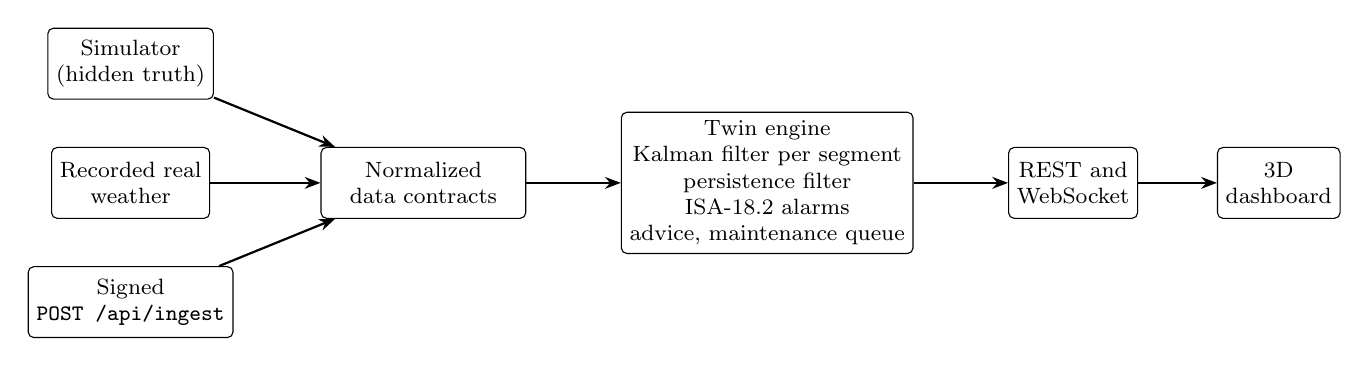
\begin{tikzpicture}[node distance=6mm and 9mm,
  box/.style={draw,rounded corners=2pt,align=center,minimum height=9mm,inner sep=3pt,font=\footnotesize},
  arr/.style={-{Stealth[length=2mm]},thick}]
\node[box] (sim) {Simulator\\(hidden truth)};
\node[box,below=of sim] (wx) {Recorded real\\weather};
\node[box,below=of wx] (live) {Signed\\\code{POST /api/ingest}};
\node[box,right=14mm of wx,minimum width=26mm] (con) {Normalized\\data contracts};
\node[box,right=12mm of con,minimum width=36mm] (eng) {Twin engine\\Kalman filter per segment\\persistence filter\\ISA-18.2 alarms\\advice, maintenance queue};
\node[box,right=12mm of eng] (api) {REST and\\WebSocket};
\node[box,right=10mm of api] (ui) {3D\\dashboard};
\draw[arr] (sim) -- (con); \draw[arr] (wx) -- (con); \draw[arr] (live) -- (con);
\draw[arr] (con) -- (eng); \draw[arr] (eng) -- (api); \draw[arr] (api) -- (ui);
\end{tikzpicture}}
\caption{Data flow. The simulator and recorded weather feed the same data contracts used by live devices.}
\end{figure}

The twin engine consumes six typed message contracts: \code{segment\_obs}, \code{probe\_obs}, \code{vehicle\_pos}, \code{weather\_obs}, \code{incident}, and \code{maintenance}. Each message is validated for type and range on arrival. Switching between data modes does not change the twin's core logic. Three operating modes have been implemented.

\renewcommand{\arraystretch}{1.6}
\begin{center}
\small
\begin{tabularx}{\textwidth}{@{}L{2.4cm} L{5.4cm} X@{}}
\toprule
\textbf{Mode} & \textbf{Data} & \textbf{Status}\\
\midrule
Simulation & Seeded or randomised simulator, with fully reproducible outputs when a seed is given & Implemented; used for all reported results\\[6pt]
Hybrid & Simulated traffic and pavement conditions driven by a recorded real-world hourly weather series & Implemented; requires a recording run with internet access, which has not yet been completed against the live weather service\\[6pt]
Live & Devices submit batches authenticated with a shared-key HMAC & Implemented and tested using synthetic signed messages only\\
\bottomrule
\end{tabularx}
\end{center}
\renewcommand{\arraystretch}{1.35}

\subsection{Tools, licences, and deployment}
\begin{center}
\small
\begin{tabularx}{\textwidth}{@{}L{3.6cm} L{2.6cm} X@{}}
\toprule
\textbf{Component} & \textbf{Licence} & \textbf{Role}\\
\midrule
Python 3.12 & PSF & Programming language\\
NumPy, SciPy & BSD-3 & Numerical computation and golden-car roughness calculation\\
FastAPI, Uvicorn & MIT, BSD-3 & REST API, WebSocket, and static hosting\\
Pydantic v2 & MIT & Typed data contracts and validation\\
Three.js (included in the repository) & MIT & 3D corridor visualisation\\
pytest, httpx & MIT, BSD-3 & Automated testing\\
\bottomrule
\end{tabularx}
\end{center}

The system provides a REST API for state queries, segment history, run control, and operator actions; a WebSocket stream that updates four times per second; and a signed data-ingestion interface. The prototype is launched from the project root with a single command and is viewed in a web browser on the same computer, without any network connection. A container image is also provided. All software components are available without licence fees.

\subsection{Dashboard}
The dashboard provides a 3D representation of the corridor, a segment list, an alarm list with acknowledgement controls, rerouting advice, a maintenance queue with work-order functionality, and a per-segment panel displaying condition history. The history chart can also overlay the simulator's hidden ground truth for evaluation purposes. Following ISA-101 principles \cite{isa101}, colour is reserved for abnormal conditions. The road width is exaggerated in the 3D view to improve visibility.

Each simulation run begins with a dialog in which the user may select up to three scenarios to run together (heavy rain, overloaded trucks, traffic surge, road closure, accident, and sensor outage) or none. A bar below the header shows which scenarios are active and how much time remains for each. A fourth scenario is refused, and the same scenario cannot be active twice. A run can be paused, and it can be stopped, after a confirmation, which discards its state and returns to the dialog so that a fresh run can be started. Ten simulation speeds are available, from 10 simulated minutes per second to two simulated days per second. Each run starts from a new random road, with different worn sections and potholes. The seed of the run is displayed, and entering it again repeats the run.

\begin{figure}[h]
\centering
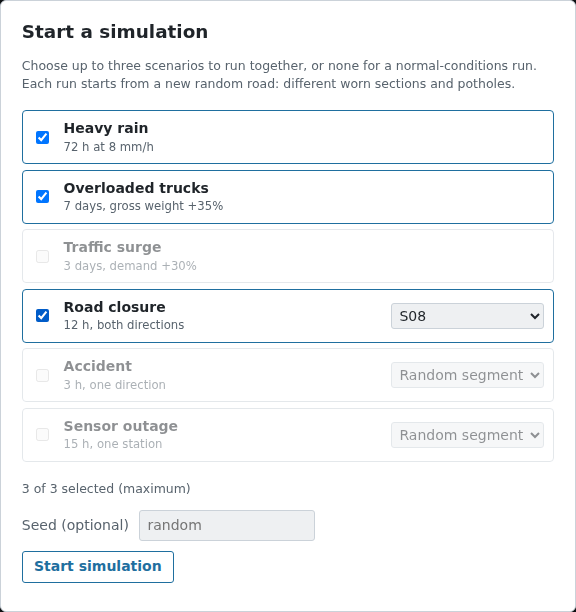
\includegraphics[width=0.62\textwidth]{figures/dashboard_setup.png}
\caption{Start dialog. Up to three scenarios can be selected together, with an optional seed. Simulated data.}
\end{figure}
\begin{figure}[h]
\centering
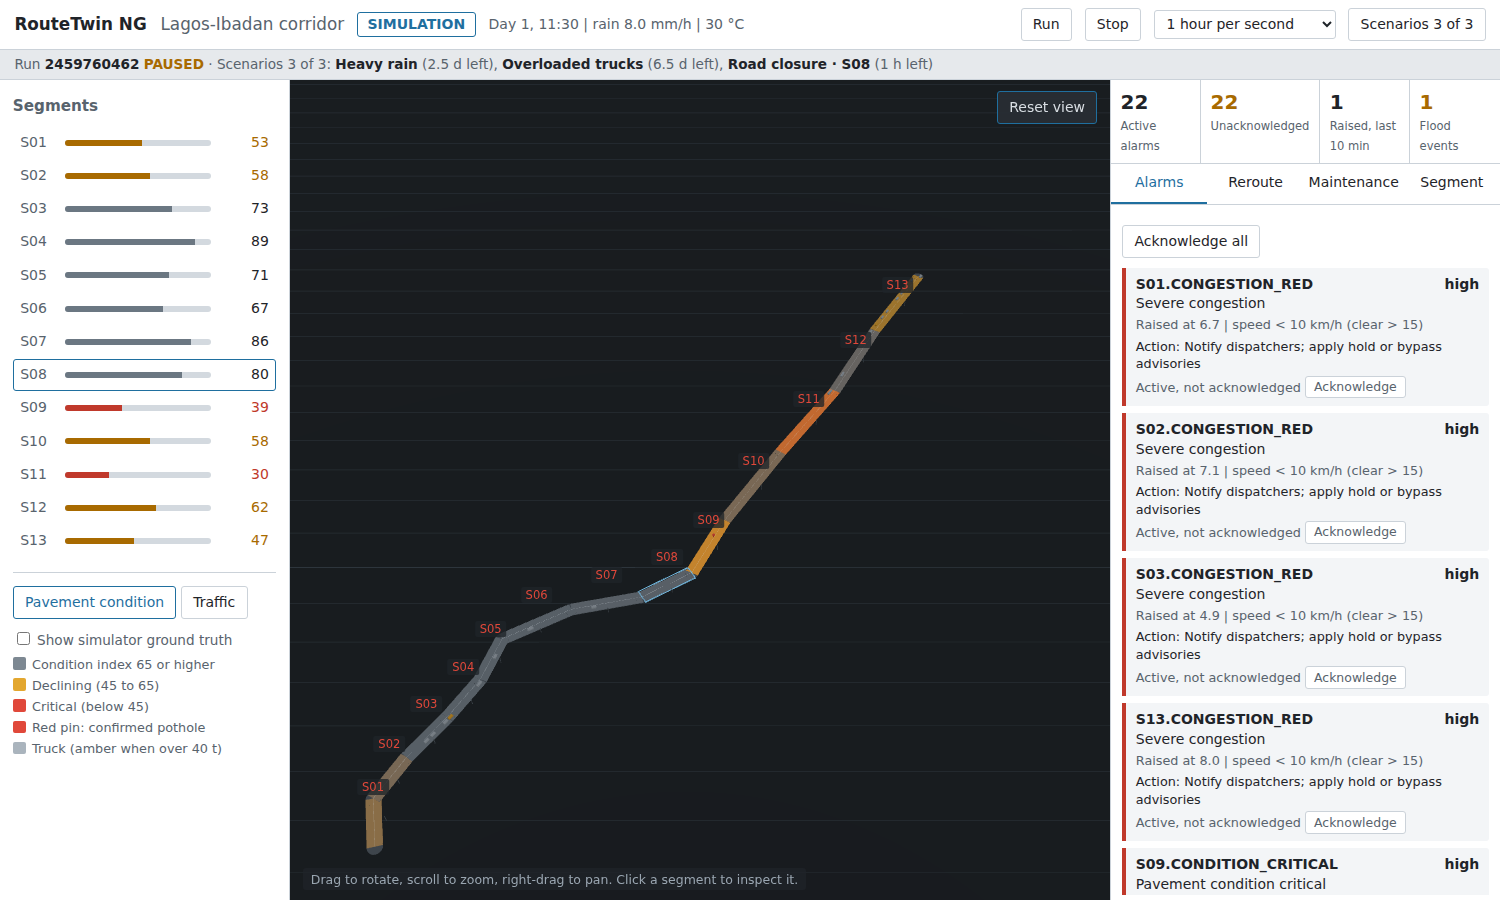
\includegraphics[width=\textwidth]{figures/dashboard_condition.png}
\caption{Condition layer. Critical segments are shown in red, declining segments in amber, and all other segments in neutral grey. Simulated data.}
\end{figure}
\begin{figure}[h]
\centering
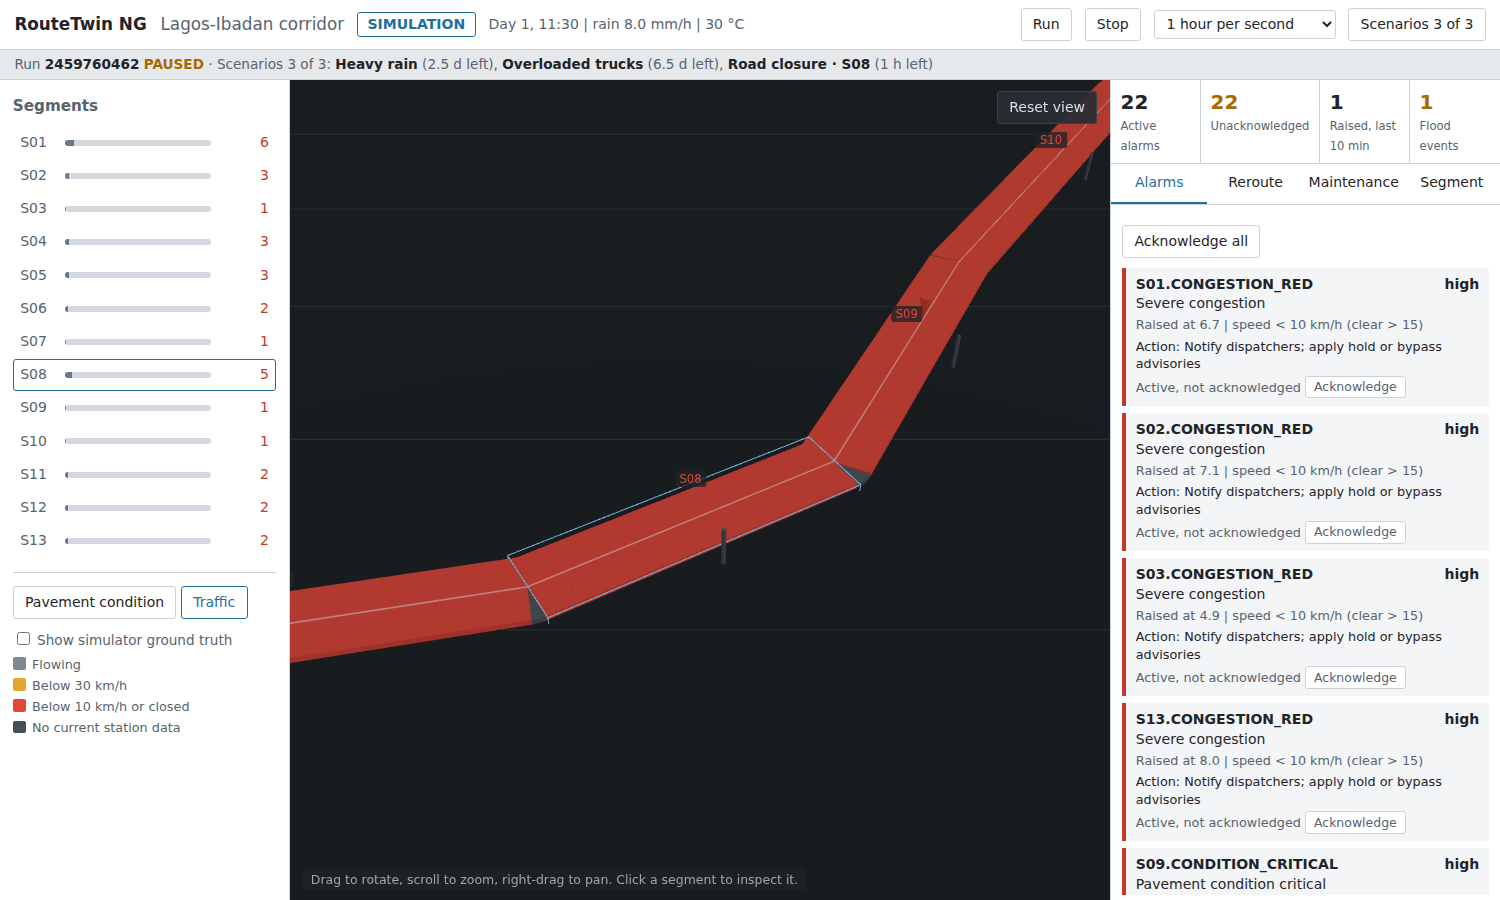
\includegraphics[width=\textwidth]{figures/dashboard_traffic.png}
\caption{Traffic layer with heavy rain, overloaded trucks, and a closure of segment S08 running together. Queues propagate upstream and severe-congestion alarms are raised. Simulated data.}
\end{figure}

%==========================================================================
\section{Practical workability}\label{sec:workability}
\subsection{Equipment and cost estimate for a three-station pilot}
To progress from simulation to a real-world deployment, we propose instrumenting three sites: one at a bottleneck, one on a deteriorated section, and one on a section in good condition. Each site would require a weigh-in-motion system, a pavement temperature probe, and a small solar-powered unit for transmitting data over a mobile network. The weigh-in-motion systems would be specified and tested against ASTM E1318 \cite{astm1318}.

The cost estimate has two parts. The civil and installation works at each station were priced item by item from published Nigerian rate books. The unit rates are taken from the Buildocrat rate book of October 2026, which is based on Abuja and excludes contractor overheads and profit \cite{buildocrat}, and the exchange rate used is the \mbox{NGN\,1,365} per US dollar published on the same site. The BuildMNO rate card for the fourth quarter of 2026 takes Lagos and the South West as its baseline and reports Abuja rates as 1.2 to 1.3 times higher \cite{buildmno}, so the Abuja-based rates used here may overstate costs along the Lagos--Ibadan corridor by about 20\%. No downward adjustment was applied. Allowances were added for contractor overhead and profit (15\%), value-added tax (7.5\%), price escalation (15\%, consistent with the all-items inflation rate of 14.63\% reported by the National Bureau of Statistics \cite{nbs}), contingency (15\%), and professional fees and project management (5\% of the net works cost, at the lower ends of the BuildMNO ranges). None of the sources consulted publishes prices for weigh-in-motion equipment, so the equipment costs are planning allowances and not quotations. They are marked as assumed in the tables and must be replaced by vendor quotations before any commitment.

\renewcommand{\arraystretch}{1.3}
\begin{table}[h]
\centering\scriptsize
\begin{tabularx}{\textwidth}{@{}X l r l r r@{}}
\toprule
\textbf{Item} & \textbf{Code} & \textbf{Qty} & \textbf{Unit} & \textbf{Rate (NGN)} & \textbf{Amount (NGN)}\\
\midrule
Break up existing pavement for sensor slots (150 mm slab, six lanes) & H02 & 36 & m$^2$ & 16\,942 & 609\,912\\
Reinforced concrete 1:2:4 for sensor frames and cabinet base & B02 & 11 & m$^3$ & 127\,723 & 1\,404\,953\\
Asphalt wearing course, 50 mm, reinstatement & R06 & 36 & m$^2$ & 20\,481 & 737\,316\\
Tack coat & R05 & 36 & m$^2$ & 420 & 15\,120\\
Cable trench by backhoe & A09 & 48 & m$^3$ & 5\,277 & 253\,296\\
Backfill and compaction of trench & A04 & 48 & m$^3$ & 2\,899 & 139\,152\\
Armoured power cable, 16 mm$^2$, four-core, laid & F25 & 150 & m & 24\,027 & 3\,604\,050\\
Earthing set (rod, conductor, inspection pit) & F27 & 2 & nr & 69\,839 & 139\,678\\
5 kVA hybrid solar system with battery, installed & F32 & 1 & nr & 4\,960\,450 & 4\,960\,450\\
Precast concrete safety barrier around the cabinet & R23 & 30 & m & 105\,047 & 3\,151\,410\\
Retro-reflective road sign on post & R26 & 4 & m$^2$ & 137\,810 & 551\,240\\
Thermoplastic road marking, 100 mm line & R12 & 200 & m & 711 & 142\,200\\
Setting out by surveyor and two chainmen & Z08 & 3 & day & 65\,237 & 195\,711\\
Asphalt core and extraction tests & Z14 & 6 & nr & 40\,000 & 240\,000\\
IP CCTV camera with cable and recorder share & X16 & 2 & nr & 113\,384 & 226\,768\\
\midrule
Net subtotal & & & & & 16\,371\,256\\
Contractor overhead and profit (15\%) & & & & & 2\,455\,688\\
VAT (7.5\%) & & & & & 1\,412\,021\\
Price escalation (15\%) & & & & & 2\,824\,042\\
Contingency (15\%) & & & & & 2\,824\,042\\
Professional fees and project management (5\% of net) & & & & & 818\,563\\
\midrule
\textbf{Local works per station} & & & & & \textbf{26\,705\,611}\\
\bottomrule
\end{tabularx}

\caption{Civil and installation works for one station. Codes refer to items in the Buildocrat rate book \cite{buildocrat}; quantities are our estimates for a dual three-lane carriageway.}
\end{table}
\begin{table}[h]
\centering\small
\begin{tabularx}{\textwidth}{@{}X r@{}}
\toprule
\textbf{Item} & \textbf{USD}\\
\midrule
Local civil and installation works, three stations (NGN~26\,705\,611 each at NGN~1\,365/USD) & 58\,694\\
Imported equipment, three stations (USD 33\,000 each plus 15\% contingency; \emph{assumed}) & 113\,850\\
Instrumented probe loggers (five, phone or inertial) & 1\,500\\
Reference profilometer surveys (two campaigns) & 10\,000\\
Static axle-scale checks of the stations & 3\,000\\
Pilot server and uninterruptible power supply & 2\,500\\
\midrule
\textbf{Total} & \textbf{189\,500}\\
\bottomrule
\end{tabularx}

\caption{Estimated budget for the three-station pilot. The total is dominated by the equipment allowance, which is the least certain item, so we regard it as accurate to about $\pm$40\%.}
\end{table}
\renewcommand{\arraystretch}{1.35}

Engineering and calibration labour would be contributed by the project team and is not included. The estimate also excludes sensor maintenance and recalibration during the pilot, which can be significant for weigh-in-motion sensors in heavy traffic. Instrumented probe trucks would require one inertial logger each, although phone-based loggers would be sufficient for initial trials. Lower-cost starting points are also possible, including reusing data from existing weighbridges and conducting manual traffic counts.

\subsection{Implementation steps and schedule}
\begin{center}
\small
\begin{tabularx}{\textwidth}{@{}L{1.8cm} L{2.4cm} X@{}}
\toprule
\textbf{Phase} & \textbf{Months} & \textbf{Work}\\
\midrule
0 & Complete & Prototype, simulator, dashboard, and automated tests\\[4pt]
1 & 1--2 & Engage the road owner and operators, agree on pilot sites, establish data-access and security requirements, and request quotations\\[4pt]
2 & 3--5 & Procure and install the three stations, commission the communication links, and calibrate the probe vehicles against profilometer surveys\\[4pt]
3 & 6--8 & Operate in shadow mode and calibrate $N_{\mathrm{design}}$, $f_T$, $f_W$, $\beta$, the roughness-to-condition relationship, and the traffic parameters against measured data\\[4pt]
4 & 9--14 & Validate performance across a rainy season using profilometer surveys and static scale checks, followed by an acceptance review\\
\bottomrule
\end{tabularx}
\end{center}

\subsection{Risks}
\begin{center}
\small
\begin{tabularx}{\textwidth}{@{}L{4.4cm} X@{}}
\toprule
\textbf{Risk} & \textbf{Mitigation}\\
\midrule
Model parameters do not match real pavement behaviour, and the absolute condition estimate is sensitive to the roughness-to-condition curve (Section~\ref{sec:results}) & Calibrate during Phase 3 against reference surveys; state thresholds in IRI, which is measured directly; retain simulated labels for results until field validation is complete\\[4pt]
Sensor accuracy drifts with temperature or speed & Conduct static scale checks, declare the accuracy class in the WIM specification, and use stale-data alarms to suppress dependent alarms\\[4pt]
Site access, theft, and vandalism & Agree on roadside cabinet locations with the road operator, use hardened solar-powered equipment, and implement remote equipment-health alarms\\[4pt]
Power and network outages & Buffer data at the edge and upload it in batches; use replay protection that accommodates delayed batches within the permitted freshness window\\[4pt]
Cybersecurity risks to telemetry & Use signed batches, operator tokens, and audit logs, and refuse to start in unsecured modes outside simulation (Section~\ref{sec:standards})\\[4pt]
Alarm overload during major events & Apply priorities, deadbands, on-delays, suppression rules, and alarm-flood monitoring\\
\bottomrule
\end{tabularx}
\end{center}

\subsection{Testing plan}
\begin{enumerate}
\item \textbf{Software verification (completed).} The 61 automated tests cover load equivalency, roughness computation, estimator convergence and outlier rejection, the alarm lifecycle, contract validation, signature and replay checks, API behaviour, determinism, scenario responses, and the run controls (random seeds, the three-scenario limit, scenario expiry, and stopping and restarting a run).
\item \textbf{Simulated scenarios and estimator validation (completed).} Closure, accident, overloading surge, heavy rain, traffic surge, sensor outage, and maintenance scenarios have been simulated and checked against the expected alarms and system states. Filter-consistency and model-mismatch runs are reported in Section~\ref{sec:results}.
\item \textbf{Bench tests (planned).} Station sensors and the gateway will be tested against reference instruments before installation.
\item \textbf{Field validation (planned).} We propose the following targets, subject to agreement with the road owner: mean absolute roughness error below 0.7~m/km relative to profilometer surveys; weigh-in-motion accuracy within the declared class during static scale checks; detection of severe congestion within 20 minutes of onset relative to manual observations; and alarm performance consistent with ISA-18.2 and EEMUA 191 guidance, with infrequent alarm-flood events \cite{eemua191}.
\end{enumerate}

Simulated and field results will be stored and reported separately, using \code{data/simulated} and \code{data/field} in the repository, respectively.

%==========================================================================
\section{Standards and originality}\label{sec:standards}
Standards are important because the twin's alarms may inform decisions by people responsible for road operations and maintenance. We have used relevant standards as design guidelines and developed tests to check whether the implementation follows the intended principles.

The standards below are applied to the relevant areas of the design. Where a standard was developed for a different domain, its application is described as an analogy. We do not claim formal certification or compliance.

\begin{center}
\scriptsize
\renewcommand{\arraystretch}{1.5}
\begin{longtable}{@{}L{2.4cm} L{5.0cm} L{3.7cm} L{3.7cm}@{}}
\toprule
\textbf{Standard} & \textbf{Design choice} & \textbf{Where} & \textbf{Evidence}\\
\midrule
\endhead
ISA-18.2 \cite{isa182} & Each alarm has a priority, setpoint, deadband, on-delay, consequence, and operator action. The lifecycle runs from active-unacknowledged to return-to-normal. Slow traffic is a display state rather than an alarm. Suppression by design prevents a closure from generating redundant congestion alarms nearby, a critical condition from generating maintenance-due alarms, and stale data from triggering dependent alarms. Alarm-flood and standing-alarm indicators are also provided. & \code{routetwin/alarms.py}, alarm definitions in \code{routetwin/twin.py} & Alarm lifecycle, suppression, and flood tests; closure scenario test\\[6pt]
ISA-101 \cite{isa101} & Neutral display, colour reserved for abnormal states, consistent navigation, visible keyboard focus, and a confirmation before an action that discards a run & \code{web/style.css}, \code{web/app.js} & Inspection; no automated test\\[6pt]
ISA/IEC 62443-3-3 \cite{iec62443}, selected requirements & In live mode: HMAC-signed telemetry for identification, integrity, and replay protection; operator tokens; strict typed validation; audit logging; and refusal to start unsecured outside simulation. Not implemented: roles, zones and conduits, key management, and encryption, which would be provided by the host's TLS & \code{routetwin/security.py}, \code{runtime.py}, \code{api.py} & Signature, replay, validation, and live-mode API tests\\[6pt]
ISA-95 \cite{isa95} & Completed work orders are exchanged as typed maintenance events, while the maintenance queue provides an interface to an asset management system. This applies the information-model concept rather than implementing the full standard. & \code{routetwin/contracts.py}, \code{decision.py} & Maintenance reset test\\[6pt]
ISO 13374-1 \cite{iso13374}, by analogy & Acquisition, processing, state detection, health assessment, prognosis, and advisory generation & \code{twin.py}, \code{estimator.py}, \code{decision.py} & Estimator and system tests\\[6pt]
ISO 8608 \cite{iso8608} with IRI \cite{sayers,astm1926} & Golden-car roughness computation checked using synthetic profiles of known class; simulated IRI values by class: A 2.1, B 4.3, C 8.6, D 17.2 m/km & \code{routetwin/iri.py} & Class-ordering and linearity tests\\[6pt]
AASHTO 1993 \cite{aashto} & Fourth-power load equivalency for each axle group & \code{routetwin/pavement.py} & Fourth-power and overloading tests\\[6pt]
Nigeria Data Protection Act 2023 \cite{ndpa} & Driver identities are not required, vehicle identifiers are opaque and optional, and a retention policy will be established for any pilot. The policy has not yet been enforced in code. & Contracts & Design statement\\
\bottomrule
\end{longtable}
\end{center}

ISA-88 (batch control) and ISA-84 (functional safety) are not applicable to the proposed system because the twin is advisory, has no trip function, and does not control a batch process.

\textbf{Alarm rationalisation.} In the prototype, pavement-condition alarms (condition critical and maintenance due) are raised through the same alarm manager as congestion and closure so that the complete alarm lifecycle can be demonstrated. Under a full ISA-18.2 rationalisation, these slow-changing conditions would be reclassified as advisories or notifications, because no operator response is required within minutes, and only events such as congestion and closure would remain alarms. The pilot would include this rationalisation with the road operator.

\subsection{Original contribution}
The underlying methods---fourth-power load equivalency, Kalman filtering, and cell-transmission traffic modelling---are established techniques. Our contribution lies in their integration and application within an industrial digital twin for road infrastructure.

\begin{itemize}
\item A pavement twin that combines load-driven predictions with roughness measurements from passing vehicles and estimates a structural-response multiplier for each segment.
\item A persistence filter that converts noisy bump events into confirmed, geolocated potholes, with no false entries observed in simulation.
\item An ISA-18.2- and ISA-101-informed approach to infrastructure-twin operation, including suppression rules for consequential traffic alarms.
\item A common data contract for simulation, hybrid, and live operating modes, supported by verification against hidden simulated ground truth and an explicit distinction between simulated and field evidence.
\end{itemize}

We have not yet completed the literature review required to establish whether this combination is novel relative to existing systems. We therefore make no claim that it is the first of its kind.

%==========================================================================
\section{Simulation results}\label{sec:results}
We evaluated the twin against a simulated road whose true condition was hidden from the estimator, measuring the accuracy of its estimates. We then tested the effect of an incorrect model and compared alternative strategies for allocating the same maintenance budget. All results in this section are simulated.

\subsection{Estimation accuracy}
When the simulated truth follows the same model family as the twin, the mean absolute condition-index error was 0.26 points after 30 simulated days using the scripted demonstration scenario, between 0.34 and 0.40 points across the 180-day maintenance simulations, and 0.50 points over 60 days with an overloading surge in the validation runs described below (mean of three seeds). The load multiplier $\theta$ had not been fully recovered after 30 days. The pothole registry matched the ground-truth count in every segment.

\subsection{Filter consistency and model mismatch}
Two further checks address the limitation of testing a model against itself. First, the mean normalised innovation squared (NIS) of the filters should be close to 1 if their stated uncertainty matches their actual errors. Second, in a mismatched case, the simulated truth uses a different load exponent (3.2 instead of 4) and a different roughness curve ($\beta=1.6$ and a span of 6 instead of 1.3 and 7), and the twin is not informed of this. The truth parameters were chosen by the authors and are not derived from data. Both cases include an overloading surge on day 20, and results are averaged over three seeds and 60 days after a 10-day burn-in.

\begin{table}[h]
\centering\small
\renewcommand{\arraystretch}{1.4}
\begin{tabular}{lrrrr}
\toprule
Case & CI MAE & CI bias & Truth within 2 SD & Mean NIS\\
\midrule
Matched truth & 0.50 & -0.19 & 64\% & 1.13\\
Mismatched truth & 12.30 & +12.30 & 0\% & 1.13\\
\bottomrule
\end{tabular}

\caption{Estimator validation (simulated). CI error is expressed in condition-index points, bias is the estimate minus the truth, and ``within 2 SD'' is the share of segment-days on which the true CI lay within two of the twin's reported standard deviations.}
\end{table}

Three conclusions follow. First, with matched models, the filter's NIS is 1.13, close to the ideal value of 1, and the error is small. However, the true value lay within two reported standard deviations on only 64\% of segment-days, where approximately 95\% would be expected, so the uncertainty bands reported by the twin are too optimistic and should not be presented as confidence intervals. Second, with mismatched models, the NIS remains at 1.13, so a filter that appears consistent does not reveal the problem, and the twin overestimates condition by 12.3 points on average, concluding that the road is in better condition than it actually is. Third, the absolute condition index therefore depends on the roughness-to-condition relationship, and only independent reference measurements can calibrate it. Roughness itself is measured directly, so decisions based on IRI thresholds are less exposed to this error. This is why the pilot includes calibration of that relationship (Phase 3) and why the field target in Section~\ref{sec:workability} is stated as a roughness error.

\subsection{Maintenance policy comparison}
All policies except ``none'' receive the same budget: 12 units per 30 days, with unused funds accumulating over time. Patching costs 1 unit and resurfacing costs 12 units. Each policy is evaluated over 180 days using identical simulated weather, demand, and incident conditions, with results averaged over two random seeds. The ``Fixed'' policy resurfaces segments in rotation. ``Oracle inspection'' is an optimistic baseline that knows the true pavement condition and the location of every pothole at no cost, with inspections every 30 days. The ``Twin'' policies use estimated conditions and make decisions every 30 or seven days.

\begin{table}[h]
\centering\small
\renewcommand{\arraystretch}{1.4}
\begin{tabular}{lrrrr}
\toprule
Policy & Mean CI & Segment-days CI$<$45 & Pothole-days & Spend (units)\\
\midrule
None & 54.3 & 704 & 1597 & 0\\
Fixed rotation & 62.3 & 574 & 1038 & 72\\
Oracle inspection, 30 d & 65.8 & 268 & 212 & 62\\
Twin, 30 d & 66.1 & 280 & 246 & 66\\
Twin, 7 d & 66.2 & 289 & 222 & 61\\
\bottomrule
\end{tabular}

\caption{Simulated maintenance-policy comparison (matched models). Lower values are better, except for mean CI, where higher is better. Only two random seeds were used, so variability across seeds has not been characterised. Results depend on illustrative parameters, including the assumed cost ratio of 1 to 12 and the assumption that resurfacing restores damage to 0.05.}
\end{table}

\textbf{Interpretation.} The twin performs approximately as well as the oracle-inspection policy when both operate with the same budget and decision cadence. This is consistent with the twin's estimates being accurate within the simulated model. Both policies outperform calendar-based rotation, although the fixed baseline cannot patch potholes. Consequently, part of the performance gap reflects the maintenance strategy itself---condition-based targeting and lower-cost patching---rather than the twin alone.

Increasing the decision frequency from every 30 days to every seven days made little difference in this simulation. Weekly decisions produced slightly fewer pothole-days but did not reduce the number of segment-days spent below CI 45. The twin's potential practical advantage over inspection is that it may reduce the need for dedicated inspection campaigns, which are assigned no cost in this simulation. Only field validation can establish whether a real-world performance improvement exists and, if so, its magnitude.

%==========================================================================
\section{Limitations}
\begin{itemize}
\item No field data are available yet. All parameters---including road capacities, design ESALs, damage and speed coefficients, hazard rates, and bypass options---are illustrative placeholders. The corridor waypoints are also approximate.
\item The simulated traffic demand is an uncalibrated assumption of approximately 75,000 vehicles per day across both directions, and published estimates for the corridor vary widely.
\item The simulator generates pavement ground truth using the same model family as the twin. Consequently, the reported estimation accuracy for the matched case is likely optimistic relative to performance under real-world model mismatch, which the mismatch test shows can dominate the error.
\item The uncertainty reported by the twin is overconfident, and the absolute condition index depends on the roughness-to-condition curve.
\item The assumptions listed in Section~\ref{sec:assumptions} (probe calibration, weigh-in-motion error, flexible pavement, station sharing, and fixed road features) have not been tested.
\item The roughness computation omits the standard 250~mm moving-average pre-filter.
\item The equipment costs in the pilot budget are planning allowances, and the civil works rates are taken from published rate books and have not been confirmed by contractor quotations.
\item Dashboard advice is generic to each segment and relies on bypass options that remain placeholders.
\item The scripts for recording weather data and retrieving OpenStreetMap geometry have not yet been run against the live services, and the dashboard was checked in a headless browser with software rendering.
\end{itemize}

\section{Conclusion}
RouteTwin NG demonstrates, through a working prototype, how a smart-road digital twin can combine truck axle loads, roughness measurements, and traffic speeds to estimate pavement condition, locate potholes, generate alarms informed by ISA-18.2, and prioritise maintenance actions. The proposal distinguishes demonstrated software behaviour from real-world performance: the current evidence comes from a verified simulation whose weaknesses have been tested and reported, while a three-station pilot on the Lagos--Ibadan expressway provides a defined path towards field validation.

\appendix
\section{Mapping to the judging framework}
\renewcommand{\arraystretch}{1.5}
\begin{center}
\small
\begin{tabularx}{\textwidth}{@{}L{4.4cm} X@{}}
\toprule
\textbf{Criterion} & \textbf{Where addressed}\\
\midrule
Problem relevance & Section 1: challenges, asset, evidence on axle overstress, and measurable objectives\\
Technical understanding & Section 2: load, damage, state estimation, traffic, instrumentation, and the assumptions in Section 2.7\\
Innovation & Section 5.1 and the update method in Section 2.3\\
Feasibility & Section 4: equipment, sourced cost estimate, schedule, risks, and pilot; open-source software stack\\
Data and modelling approach & Sections 2.1 to 2.3, the three data modes, simulated-versus-field labelling, and Section 6.2 on validation\\
Operational value & Section 2.6 and the policy comparison in Section 6.3\\
Presentation and communication & Layered writing, the interactive 3D dashboard (Section 3.3), and the evidence labels\\
\bottomrule
\end{tabularx}
\end{center}

\renewcommand{\refname}{References}
\begin{thebibliography}{99}
\small
\setlength{\itemsep}{3pt}
\bibitem{aashto} American Association of State Highway and Transportation Officials, \emph{AASHTO Guide for Design of Pavement Structures}. Washington, DC, USA: AASHTO, 1993.
\bibitem{nbrri} Nigerian Building and Road Research Institute, ``Effect of axle loads on pavement deterioration: A case of Gombe--Numan expressway,'' NBRRI, Lagos, Nigeria. [Online]. Available: \url{https://nbrri.gov.ng/effect-of-axle-loads-on-pavement-deterioration-a-case-of-gombe-numan-expressway/} (accessed Oct.~26, 2026).
\bibitem{oguntayo} D.~O. Oguntayo, I.~T. Adelowo, and J.~K. Olaleye, ``Measurement of the traffic wheel/pavement contact characteristics for goods haulage; case study of Dangote Flour Mill PLC Ilorin, Nigeria,'' \emph{Cogent Eng.}, vol.~7, no.~1, Art.~no.~1830470, 2020, doi: 10.1080/23311916.2020.1830470.
\bibitem{pais} J.~C. Pais \emph{et al.}, ``The increase of pavement cost due to the traffic overloads,'' Univ. of Minho Repository. [Online]. Available: \url{https://www.rcaap.pt/vufind/PublicationRecord/rum_b58ae5da8b94de5bf9d90a466d4defc2} (accessed Oct.~26, 2026).
\bibitem{shippingposition} ``Apapa--Oshodi expressway completed yet impassable,'' \emph{Shipping Position}. [Online]. Available: \url{https://shippingposition.com.ng/apapa-oshodi-expressway-completed-yet-impassable/} (accessed Oct.~26, 2026).
\bibitem{businessday} ``Respite underway as Hitech mobilises for work on Apapa--Oshodi expressway,'' \emph{BusinessDay}. [Online]. Available: \url{https://businessday.ng/uncategorized/article/respite-underway-as-hitech-mobilises-for-work-on-apapa-oshodi-expressway/} (accessed Oct.~26, 2026).
\bibitem{isa182} \emph{Management of Alarm Systems for the Process Industries}, ANSI/ISA-18.2-2016, International Society of Automation, Research Triangle Park, NC, USA, 2016.
\bibitem{grieves} M.~Grieves and J.~Vickers, ``Digital twin: Mitigating unpredictable, undesirable emergent behavior in complex systems,'' in \emph{Transdisciplinary Perspectives on Complex Systems}, F.-J. Kahlen, S. Flumerfelt, and A. Alves, Eds. Cham, Switzerland: Springer, 2017, pp.~85--113.
\bibitem{iso23247} \emph{Automation Systems and Integration --- Digital Twin Framework for Manufacturing --- Part 1: Overview and General Principles}, ISO 23247-1, International Organization for Standardization, Geneva, Switzerland, 2021.
\bibitem{sayers} M.~W. Sayers, T.~D. Gillespie, and W.~D.~O. Paterson, ``Guidelines for conducting and calibrating road roughness measurements,'' World Bank, Washington, DC, USA, Tech. Paper~46, 1986.
\bibitem{astm1926} \emph{Standard Practice for Computing International Roughness Index of Roads from Longitudinal Profile Measurements}, ASTM E1926-08(2015), ASTM International, West Conshohocken, PA, USA, 2015.
\bibitem{kalman} R.~E. Kalman, ``A new approach to linear filtering and prediction problems,'' \emph{J. Basic Eng.}, vol.~82, no.~1, pp.~35--45, Mar. 1960.
\bibitem{daganzo} C.~F. Daganzo, ``The cell transmission model: A dynamic representation of highway traffic consistent with the hydrodynamic theory,'' \emph{Transp. Res. B, Methodol.}, vol.~28, no.~4, pp.~269--287, Aug. 1994.
\bibitem{isa101} \emph{Human Machine Interfaces for Process Automation Systems}, ANSI/ISA-101.01-2015, International Society of Automation, Research Triangle Park, NC, USA, 2015.
\bibitem{astm1318} \emph{Standard Specification for Highway Weigh-in-Motion (WIM) Systems with User Requirements and Test Methods}, ASTM E1318-09, ASTM International, West Conshohocken, PA, USA, 2009.
\bibitem{buildocrat} ``Building material prices and BoQ rates in Nigeria (October 2026),'' Buildocrat Rate Book. [Online]. Available: \url{https://rates.buildocrat.store/} (accessed Nov.~2, 2026).
\bibitem{buildmno} ``Nigerian construction rate card, Q4 2026,'' BuildMNO, Oct. 2026. [Online]. Available: \url{https://buildmno.com/rate-card/} (accessed Nov.~2, 2026).
\bibitem{nbs} National Bureau of Statistics, ``Consumer price index (all-items inflation rate),'' Abuja, Nigeria. [Online]. Available: \url{https://nigerianstat.gov.ng/} (accessed Nov.~2, 2026).
\bibitem{eemua191} \emph{Alarm Systems: A Guide to Design, Management and Procurement}, 3rd ed., EEMUA Publication 191, Engineering Equipment and Materials Users Association, London, U.K., 2013.
\bibitem{iec62443} \emph{Industrial Communication Networks --- Network and System Security --- Part 3-3: System Security Requirements and Security Levels}, IEC 62443-3-3:2013, International Electrotechnical Commission, Geneva, Switzerland, 2013.
\bibitem{isa95} \emph{Enterprise-Control System Integration --- Part 1: Models and Terminology}, ANSI/ISA-95.00.01-2010 (IEC 62264-1 Mod), International Society of Automation, Research Triangle Park, NC, USA, 2010.
\bibitem{iso13374} \emph{Condition Monitoring and Diagnostics of Machines --- Data Processing, Communication and Presentation --- Part 1: General Guidelines}, ISO 13374-1:2003, International Organization for Standardization, Geneva, Switzerland, 2003.
\bibitem{iso8608} \emph{Mechanical Vibration --- Road Surface Profiles --- Reporting of Measured Data}, ISO 8608:2016, International Organization for Standardization, Geneva, Switzerland, 2016.
\bibitem{ndpa} \emph{Nigeria Data Protection Act, 2023}, Federal Republic of Nigeria, 2023.
\end{thebibliography}
\end{document}
